\chapter{Logic-Based Classification}
\label{logic-based-classification}

% TODO: Alessandra feeedback
% Concept extraction can be used for a classification problem - that problem uses attention on the concepts to determine which ones are more active
% A more interpretable approach would involve rule-based classification, which we explore in this section
% Furthermore, despite the concept extraction from text presented, concepts can really be any features which is accounted for in this chapter.

In order to find reasons for choosing a particular label, the concept bottleneck pipeline \cite{RefWorks:RefID:35-koh2020concept} uses human-explainable high-level concepts in the intermediate layer.
These concepts should help a user to understand why a prediction happened.
However, just because concepts are predicted does not mean they are indeed used in the final prediction.

For example, a network may learn a pattern which predicts a label \emph{out}, if some concept has a value greater than 0.2.
Yet, such a concept would not be shown to the user as relevant for the final prediction.
Showcasing concepts after the attention layer, as we have done in the previous chapter, would showcase more relevant concepts for the final prediction.
Still, the attention layer showcases how much weight each concept has in the final prediction, but not the logic the MLP uses in order to choose the final label.

A fully interpretable method for predicting the final label would provide a clear link between the concepts and the outcomes.
In addition, model from concepts to the label can be validated and should in an ideal case follow the same logic as humans.

To improve upon the concept bottleneck model interpretability, this chapter presents a classification method using an ILP system.
The method works with probabilistic facts, allowing it to be incorporated into a concept bottleneck pipeline (Chapter \ref{concept-bottleneck-pipeline}).
Nevertheless, it is not limited to text concepts; it is applicable with any interpretable probabilistic NN output. 
% INSERT ref to evaluation
In section X, we use it with outcomes of a image classification task.
The ILP system utilised for this task is FastLAS \cite{RefWorks:RefID:19-law2020fastlas:}, a scalable system that incorporates criteria for domain-specific optimisation.

% TODO: change title
\section{Change to the Concept Bottleneck Architecture}
\label{change-to-the-concept-bottleneck-architecture}

An introduction of the rule learning component would result in the change in the concept bottleneck architecture shown in figure \ref{logic-based-concept-bottleneck}.
\begin{figure}[h]
\caption{A flowchart to select an outcome of a multi-label classification problem.}
\vspace{10pt}
\centering
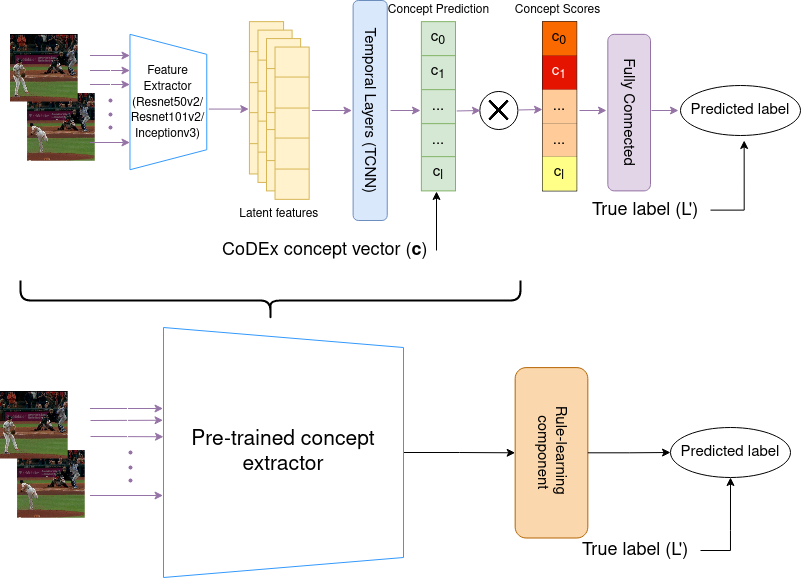
\includegraphics[width=\textwidth]{logic-based-classification/logic-based-classification-architecture.png}
\label{logic-based-concept-bottleneck}
\end{figure}

Training a concept bottleneck pipeline then turns into a 3-step process:
\begin{enumerate}
    \item Train a model in the same manner as in the Chapter \ref{concept-bottleneck-pipeline}, by minimising the loss CoDEx concept vector and final label prediction loss.
    \item Generate examples for the rule-learning component using the concepts predicted by the model from step 1). Each example needs to take into account the probabilities of all concepts.
    \item Train the rule-learning component.
\end{enumerate}

At run-time take predict the concepts using the model trained in step 1, before applying the rules learned in step 3 to obtain the final prediction.

% INSERT FF-NSL reference
The ILP paradigm does not support any notion of probability; an atom can either be in or out of an answer set. 
So, to force the learner to treat less less likely cases differently, we carefully choose the FastLAS example penalties, similar to X.
However, we aim to use those penalties to find the most likely solution.

\section{Choosing FastLAS Parameter Values}
\label{choosing-fastlas-parameter-values}

% INSERT reference to background section decomposable
FastLAS can find an optimal solution with respect to a scoring function of kind ($\curly{S} + \curly{S}_{pen}$), where $\curly{S}$ is a decomposable scoring function (X) and $\curly{S}_{pen}$ is a sum of all uncovered example penalties.

In this section, we attempt to find the appropriate scoring function $\curly{S}$ and values for penalties such that the final solution is highly likely given the learning task tuple $T = \langle B, M, E_{prob} \rangle$. 

\subsection{Used Notation}

Let our set of examples $E_{prob}$ be $\{(\vec{x}_e, y_e)\}_{e=1}^{E} \in \curly{E}$ with $E$ examples. 
An example $(\vec{x}_e, y_e)$ consist of a vector of concept probabilities $\vec{x}_e = (x_{ec})_{c=1}^C$ and a label $y_e \in \curly{L}$ assigned to the example $e$ from the set of possible labels $\curly{L}$.
The symbol $x_{ec}$ denotes a priori probability that concept $c$ takes truth value (=1) in example $e$.
Moreover, $C$ is the number of extracted concepts for a given problem. \\
We can represent examples as a matrix of concept probabilities.  
The examples can be represented as an input matrix of concept probabilities $\vec{X} = (\vec{x}_e^T)_{e=1}^E$ and an output vector of target labels $\vec{y} = (y_e)_{e=1}^E$.

Let $\curly{H}$ be the set of all possible hypotheses. The term $p(y_e|H, \vec{x}_{e})$ represents the probability that the example $e$ is covered, for any hypothesis $H \in \curly{H}$,


We introduce notation for grounded examples, as answer sets can only contain grounded atoms.
A grounded example $(\vec{z}_e, y_e)$ is an example where each concept $c$ in an example $e$ is assigned a truth value $z_{ec} \in \{0,1\}$ (integer form). 
The term $\vec{z}_e = (z_{ec})_{c=1}^C \in \curly{Z}_e$  is a binary vector representing the ground assignment. 

\subsection{Determining Optimal Example Penalties}

We want to choose the example penalties such that the FastLAS output hypothesis $H$ is the maximum-likelihood hypothesis $H_{\text{ML}}$, i.e. the output hypothesis should satisfy the following equation:
\begin{align}
H_{\text{ML}} = \arg\max_{H}
p(\vec{y}|H, \vec{X})
\end{align}

Making an assumption that given a model and concept probabilities, the labels for any two examples are conditionally independent we can rewrite the term $p(\vec{y}|H, \vec{X})$ in the following manner:
\begin{align}
p(\vec{y}|H, \vec{X})
= \prod_{e} p(y_e|H, \vec{x}_e) \label{eq6.3}
\end{align}


As the $ln = log_e$ function is monotonically increasing in the range $(0, \infty)$ and as the above equation produces values in that range, it is equivalent to maximising the $ln$, resulting in the following optimisation target:
\begin{align}
H_{\text{ML}}
& = \arg\max_{H}
\ln p(\vec{y}|H, \vec{X}) \nonumber \\
& = \arg\max_{H}
\sum_{e} \ln p(y_e|H, \vec{x}_e) && \text{(by \ref{eq6.3})} \nonumber \\
& = \arg\min_{H}
-\sum_{e} \ln p(y_e|H, \vec{x}_e) && \text{(alternative objective)} \label{ex6.4}
\end{align}


% TODO: define Z
We can now calculate the probability that a label $y_e$, for example $e$, is covered by a hypothesis $H$ where we know the set of concept probabilities $\vec{x}_e$.
That probability is computed by considering all possible grounding that $\vec{x}_e$ induces.
It is given by:
\begin{align}
p(y_e|H, \vec{x}_e)
& = \sum_{\vec{z} \in \curly{Z}_e} p(y_e, \vec{z} | H, \vec{x}_e) && \text{(sum rule)} \nonumber \\
& = \sum_{\vec{z} \in \curly{Z}_e} p(y_e | \vec{z}, H, \vec{x}_e) p(\vec{z} | H, \vec{x}_e) && \text{(conditional probability)} \nonumber \\
& = \sum_{\vec{z} \in \curly{Z}_e} p(y_e | \vec{z}, H) p(\vec{z}| \vec{x}_e) && \text{(by independence)} \nonumber \\
& = \expct_{\vec{z} \sim p(\vec{z}| \vec{x}_e)}[p(y_e|\vec{z},H)] \label{ex6.5}
\end{align}

Considering the $\ln$ of the term above, we can use the Jensen's inequality to push it inside the expectation:
\begin{align}
\ln p(y_e|H, \vec{x}_e)
&= \ln \expct_{\vec{z} \sim p(\vec{z}| \vec{x}_e)}[p(y_e|\vec{z},H)] \nonumber \\
&\leq \expct_{\vec{z} \sim p(\vec{z}| \vec{x}_e)}[\ln  p(y_e|\vec{z},H)] 
\nonumber \\
\end{align}

We further assume that the bounds of Jensen's inequality are sufficiently tight, i.e. we assume that:
\begin{align}
\ln p(y_e|H, \vec{x}_e)
&\approx \expct_{\vec{z} \sim p(\vec{z}| \vec{x}_e)}[\ln  p(y_e|\vec{z},H)] \label{jensen-approx}
\end{align}

Now we can estimate the expectation by sampling $I$ ground examples for example $e$, where ground examples are $\vec{z}_{i} \sim p(\vec{z}| \vec{x}_e)$, then:
\begin{align}
\expct_{\vec{z} \sim p(\vec{z}| \vec{x}_e)}[\ln  p(y_e|\vec{z},H)]
\approx \frac{1}{I} \sum_{i=1}^{I} \ln  p(y_e|\vec{z}_i,H) \label{sampling-result}
\end{align}


For some hypothesis, $H\in \curly{H}$, a grounded example is or is not covered by $H$. We allow a label to be incorrect with some small error $\epsilon > 0$, resulting in the following probabilistic interpretation:
\begin{align}
p(y_e | \vec{z}, H) =
\begin{cases}
1 - \epsilon & \text{if } H, \vec{z} \models y_e \\
\epsilon & \text{otherwise}
\label{def-ground}
\end{cases}
\end{align}

Combining all the results presented, we can derive the following:
\begin{align}
H_{\text{ML}}
& = \arg\min_{H} 
-\sum_e \ln \left( \expct_{\vec{z} \sim p(\vec{z}| \vec{x}_e)}[p(y_e|\vec{z},H)] \right ) 
&& \text{(by \ref{ex6.4} and \ref{ex6.5})} \nonumber \\
& \approx \arg\min_{H}
-\sum_e \expct_{\vec{z} \sim p(\vec{z}| \vec{x}_e)}[\ln \left[ p(y_e|\vec{z},H) \right ]]  
&& \text{(by \ref{jensen-approx})} \nonumber \\
& \approx \arg\min_{H}
\sum_e \frac{1}{I} \sum_{i=1}^I -\ln \left[ p(y_e|\vec{z},H) \right ]
&& \text{(by \ref{sampling-result})} \nonumber \\
& = \arg\min_{H} \sum_e \frac{1}{I} \sum_{i=1}^I  \left(-\ln  [p(y_e|\vec{z}_{ei},H)] + \ln (1-\epsilon) \right)
&& \text{(constant shift)} \nonumber \\
& = \arg\min_{H}
\sum_e \frac{1}{I} 
\left (
\sum_{H,\vec{x}_{ei}\models y_e} 0
+
\sum_{H,\vec{x}_{ei}\not\models y_e} (-\ln \epsilon + \ln (1 - \epsilon))
\right ) 
&& \text{(by \ref{def-ground})} \nonumber \\
& = \arg\min_{H}
\sum_e  
\sum_{H,\vec{x}_{ei}\not\models y_e} -\frac{1}{I}\ln \left ( \frac{\epsilon}{1 - \epsilon} \right ) \label{eq-final-no-int}
\end{align}


Optimising only for the $\curly{S}_{pen}$, FastLAS would return the following solution:
\begin{align}
H
& = \arg\min_{H}
\sum_e  
\sum_{H,\vec{x}_{ei}\not\models y_e} e_{pen}
\end{align}

Hence, by setting the penalty for each example to $-\frac{1}{I} \ln \left ( \frac{\epsilon}{1 - \epsilon} \right )$ and prior penalties to 0, FastLAS would return a solution close to the maximum likelihood for all examples.

\subsubsection{Integer penalties}
\label{integer-penalties}

FastLAS does not support any floating point number calculations, including penalty values.

But, we can overcome this issue.
Let us consider a large value $K \in \reals^+$, and then round $K$ multiplied by each term in the sum to the nearest integer. Because for large enough $K$:
\begin{align}
    Kt \approx round(Kt) \label{rounding}
\end{align}

In addition, minimising any $t \in \reals^+$ is equivalent to minimising $K t$ for any $K \in \reals^+$.
So, the function we wish to minimise becomes: 
\begin{align}
H_{\text{ML}}
& = \arg\min_{H}
\sum_e  
\sum_{H,\vec{x}_{ei}\not\models y_e} -\frac{1}{I}\ln \left ( \frac{\epsilon}{1 - \epsilon} \right ) 
&& \text{(\ref{eq-final-no-int})} \nonumber \\
& = \arg\min_{H}
K \sum_e  
\sum_{H,\vec{x}_{ei}\not\models y_e} -\frac{1}{I}\ln \left ( \frac{\epsilon}{1 - \epsilon} \right ) 
&& \text{(scaling $t \in \reals^+$ by $K \in \reals^+$)} \nonumber \\
& = \arg\min_{H}
\sum_e  
\sum_{H,\vec{x}_{ei}\not\models y_e} -\frac{K}{I}\ln \left ( \frac{\epsilon}{1 - \epsilon} \right ) \nonumber \\ 
& = \arg\min_{H}
\sum_e  
\sum_{H,\vec{x}_{ei}\not\models y_e} \text{round} \left ( -\frac{K}{I}\ln \left ( \frac{\epsilon}{1 - \epsilon} \right ) \right )
&& \text{(by \ref{rounding})}
\end{align}

Therefore, after choosing some large $K > 0$, we assign the non-coverage penalty of $\text{round} \left ( -\frac{K}{I} \ln \left ( \frac{\epsilon}{1 - \epsilon} \right ) \right )$ for each example.

\subsection{Incorporating a Prior over the Hypothesis Space}

Now, we can extend the approach done in the previous section by considering a prior over hypothesis space ($p(H)$) too.
The extension would give a plausibility value to each potential $H$ before we evaluate its fitness on the examples. 
We can combine this with the likelihood function to give a posterior probability for the data and hypothesis, namely:
\begin{align}
p(\vec{y}, H|\vec{X})
& = p(\vec{y}|H, \vec{X})p(H)
\end{align}

We can log this to get:
\begin{align}
\ln p(\vec{y}, H|\vec{X})
& = \ln p(\vec{y}|H, \vec{X}) + \ln p(H)
\end{align}

Maximising the above equation leads to what we would call the maximum posterior estimate for $H$, or maximum a posteriori (MAP) estimate:
\begin{align}
H_{\text{MAP}}
& = \arg\max_{H} \ln p(\vec{y}|H, \vec{X}) + \ln p(H) 
\end{align}

% As with the maximum likelihood approach we can maximise the rescaled expression using $K \in \reals^+$ giving:
% \begin{align}
% h_{\text{MAP}}
% & = \arg\max_{h} \left(K\ln p(\vec{y}|h, \vec{X}) + K\ln p(h) \right)
% \end{align}

% Or we can see this as minimising a negative log-loss:
% \begin{align}
% h_{\text{MAP}}
% & = \arg\min_{h} \left(-K\ln p(\vec{y}|h, \vec{X}) - K\ln p(h) \right)
% \end{align}

% Note the important point here is that the scale of the penalties on the prior must match the scale of penalties on the examples.

\subsubsection{Choosing a Meaningful Prior over the Hypothesis Space}

There are several ways to place a prior on hypothesis space. 
The default ILASP \cite{RefWorks:RefID:18-law2020ilasp} and the usual FastLAS approach assign smaller penalties, i.e., higher prior probabilities, to shorter clauses.
% INSERT online symbolic learning of policies for explainable security
Some problems benefited from assigning lower penalties to "ideal length" rules, such as X.

We have opted for a slightly different approach. \\
Starting with a set of potential rules $\curly{R}$, let $q_r$ be an independent probability that $r$ is included in $H$ (written $r \in H$) for every potential rule $r \in \curly{R}$. Then the prior is written as:
\begin{align}
p(H) = \left(\prod_{r \in H} q_r\right)\left(\prod_{r \in \curly{R}\setminus H} (1-q_r)\right)
\end{align}

We can log this for convenience:
\begin{align}
\ln p(H) = \sum_{r \in H} \ln q_r + \sum_{r \in \curly{R}\setminus H} \ln(1-q_r) \label{log-prior-rule}
\end{align}


For a fixed reference hypothesis such as $H_0 = \emptyset$, maximising the posterior is equivalent to maximising the posterior divided by the prior, resulting in:
\begin{align}
H_{\text{MAP}}
& = \arg\max_{H} p(\vec{y}|H, \vec{X}) p(H)  \nonumber \\
& = \arg\max_{H} \left(\frac{ p(\vec{y}|H, \vec{X}) p(H)}{p(H_0)}\right)  \nonumber \\
& = \arg\min_{H} \left( -K\ln p(\vec{y}|H, \vec{X}) - K \ln \frac{p(H)}{p(H_0)}\right) \label{h-map-final}
\end{align}
The above equation holds for some $K > 0$, added to deal with FastLAS inability to work with non-integers as in \ref{integer-penalties}.

The ratio of the overall change in prior for any hypothesis $H \in \curly{H}$ from the empty hypothesis $H_0 = \emptyset$ can then be calculated using \ref{log-prior-rule} as follows:
\begin{align}
\ln \left(\frac{p(H)}{p(H_0)}\right) 
& = \sum_{r \in H} \ln q_r + \sum_{r \in \curly{R}\setminus H} \ln(1-q_r) \nonumber
- \sum_{r \in \emptyset} \ln q_r - \sum_{r \in \curly{R}} \ln(1-q_r) \\
& = \sum_{r \in H} \left(\ln q_r - \ln(1-q_r) \right)
\end{align}

As FastLAS finds an optimal solution with respect to the scoring function ($\curly{S}_{pen} + \curly{S}$), it can satisfy the equation \ref{h-map-final} if we choose the examples penalties as in \ref{integer-penalties} and the following $\curly{S}$:
\begin{align}
    \curly{S}(H, T) =  -K \sum_{r \in H} \left(\ln q_r - \ln(1-q_r) \right)
\end{align}
By inspection, we see that the decomposition of the function $\curly{S}$ is given by:
\begin{align}
    \curly{S}^{rule}(r, T) = -K (\ln q_r - \ln(1-q_r))
\end{align}


Finally, we need to choose appropriate values probabilities $q_c$. \\
Imagine that we have a rule of length $l$, we would expect to find $m_l$ clauses of length $l$ in a specific hypothesis, and there are $n_l$ clauses of length $l$ in the set of all possible rules $\curly{R}$. 
This setup suggests a value for $q_{r_l} = \frac{m_l}{n_l}$, resulting in the following change to the $\curly{S}^{rule}$:
\begin{align}
\curly{S}^{rule}(r, T) 
& = -K (\ln q_r - \ln(1-q_r)) \nonumber \\
& = -K \left (\ln \frac{m_l}{n_l} - \ln \frac{n_l - m_l}{n_l} \right) \nonumber \\
& = K \left (\ln (n_l - m_l) - \ln m_l  \right)
\end{align}

\section{Implementation}

% TODO: merge binary classification and multi-label classification into one subsection
\subsection{Encoding Binary Classification Task}
\label{encoding-binary-classification-task}

In order to encode a solution to a binary classification problem using ASP, we can do the following:
\begin{itemize}
    \item Write rules such as \verb+label1 :- ...+  for one of the labels.
    \item Add the rule of the form \verb+label2 :- not label1+.
\end{itemize}

% TODO: remove the itemise and encode is as a piece of text
With this approach, we are guaranteed to have exactly one label in each answer set of the task.
We often want exactly one answer set as a solution, as usually no reason to prefer one over the other in a classification task.
To prevent that possibility from occurring, the following types of ASP rules are not used:
\begin{itemize}
    \item Choice rules --- Choice rules give rise to multiple answer sets, which we do not want.
    \item "Not chain" --- Combination of normal rules which can only be satisfied by multiple answer sets, such as \verb+{p :- not q. q :- not p.}+.
    \item Constraints --- Constraints are used to eliminate an answer from occurring.
\end{itemize}

An alternative to this encoding which would return a solution with a highest score is also possible, however, it is not nearly as interpretable.

\begin{example}
\label{sudoku-binary-example}
Encoding the sudoku learning task:

% INSERT reference evaluation
The sudoku 4x4 learning task (X) should deduce whether a grid or is not valid.

1. \textit{Construct the background knowledge:} \\
The background knowledge for sudoku could contain the following rules that specify which row/column/block does a cell belong to.
\begin{verbatim}
num(1..4).
col(1..4).
row(1..4).
block(1..4).
% value(C, N) represents that number N is written in cell C
cell(C) :- value(C, _).

col((X, Y), Y) :- row(X), col(Y).
row((X, Y), X) :- row(X), col(Y).
block((X, Y), 1) :- row(X), col(Y), X <= 2, Y <= 2.
block((X, Y), 2) :- row(X), col(Y), X <= 2, Y > 2.
block((X, Y), 3) :- row(X), col(Y), X > 2, Y <= 2.
block((X, Y), 4) :- row(X), col(Y), X > 2, Y > 2.

neq_cell(C1, C2) :- cell(C1), cell(C2), C1 != C2.
\end{verbatim}

2. \textit{Account for the alternative label:} \\
We add the following rule to the background knowledge:
\begin{verbatim}
selected(valid) :- not selected(invalid). 
\end{verbatim}

3. \textit{Construct the language bias:} \\
We chose that we wish to learn what makes a cell invalid in this example, resulting in the following language bias:
\begin{verbatim}
#modeh(selected(invalid)).

#modeb(row(var(cell), var(row))).
#modeb(col(var(cell), var(col))).
#modeb(block(var(cell), var(block))).
#modeb(neq_cell(var(cell), var(cell))).
#modeb(value(var(cell), var(num))).

#maxv(4).
\end{verbatim}

4. \textit{Add examples and prior penalty definitions:}
% INSERT refernce to example definition and prior penalty definition
This step will be discussed in X and X.
\end{example}

\subsection{Encoding Multi-label Classification Task}

The multi-label classification outcome is decided using the flowchart in \ref{flowchart-multi-label-classification}, where the \verb_conds(label(x))_ predicate that is true when conditions for a particular label are satisfied.

\begin{figure}[h]
\caption{A flowchart to select an outcome of a multi-label classification problem.}
\vspace{10pt}
\centering
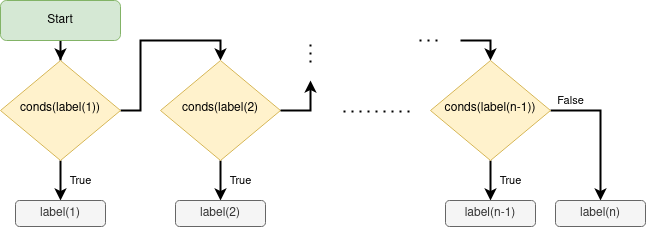
\includegraphics[width=\textwidth]{logic-based-classification/multi-label-selection.png}
\label{flowchart-multi-label-classification}
\end{figure}

The choice for the flowchart was made to aid interpretability because FastLAS learns the following set of rules:
\begin{verbatim}
conds(label(1)) :- ...
conds(label(1)) :- ...
...
conds(label(n-1)) :- ...
conds(label(n-1)) :- ...
\end{verbatim}
So, a human can easily determine the outcome by going through the rules from top to bottom and selecting a label matching the first satisfied rule.
Learning these types of rules is encoded in FastLAS with the following syntax:
\begin{verbatim}
#modeh(conds(const(learnable_label))).

... all the modeb declarations ...

% Avoid constraints
#bias("
:- constraint.
").
\end{verbatim}

Furthermore, to make the learner use the logic presented in the flowchart, we need to encode the following: 
\begin{enumerate}
    \item The position of a label in the flowchart chain.
    \item Selection the highest priority label whose conditions are satisfied.
    \item Selection of the lowest priority label when no conditions are satisfied.
\end{enumerate}
The enumerated criteria results in the following ASP encoding added to the background of a learning task:
\begin{lstlisting}
% Encoding 1 with label(name, position) (lower=better)
label(l1, 0).
label(l2, 1).
...
label(ln, n-1).

% Definitions of types for FastLAS
label(L) :- label(L, _).
learnable_label(L) :- exists_lower_priority(L, _).


% Encoding 2: Select the highest priority label whose conditions are satisfied
selected(L) :- label(L, P), conds(L), 
                 not higher_priority_selection(L, P).
higher_priority_selection(L, P) :- label(L, P), label(L2, P2), 
                                       P2 < P, selected(L2).

% Encoding 3: Select default label if no higher priority selection is made
selected(L) :- label(L, P), not higher_priority_selection(L, P), 
                 not exists_lower_priority(L, P).
exists_lower_priority(L, P) :- label(L, P), label(L2, P2), P2 > P.
\end{lstlisting}

Notice that the presented encoding also produces exactly one answer set, same as the encoding for the binary classification.

\begin{example}
Encoding the multi-label sudoku 4x4 learning task:

% INSERT reference evaluation
Consider an extension of the binary sudoku 4x4 task in example \ref{sudoku-binary-example}, which introduces an additional label \verb_conflict_. 
That label should be true only when an example contains two digit written in the same cell.
The following steps are needed to solve the task using the presented multi-label classification encoding:

1. \textit{Construct the background knowledge:} \\
The background is the same as for example \ref{sudoku-binary-example}.

2. \textit{Add the multi-label selection encoding to the background:} \\
We add the following rules to the background knowledge:
\begin{lstlisting}
% Encoding 1 with label(name, position) (lower=better)
label(conflict, 0).
label(invalid, 1).
label(valid, 2).

% Definitions of types for FastLAS
label(L) :- label(L, _).
learnable_label(L) :- exists_lower_priority(L, _).


% Encoding 2: Select the highest priority label whose conditions are satisfied
selected(L) :- label(L, P), conds(L), 
                 not higher_priority_selection(L, P).
higher_priority_selection(L, P) :- label(L, P), label(L2, P2), 
                                       P2 < P, selected(L2).

% Encoding 3: Select default label if no higher priority selection is made
selected(L) :- label(L, P), not higher_priority_selection(L, P), 
                 not exists_lower_priority(L, P).
exists_lower_priority(L, P) :- label(L, P), label(L2, P2), P2 > P.
\end{lstlisting}

2. \textit{Construct the language bias:} \\
We chose that we wish to learn what makes a cell invalid in this example, resulting in the following language bias:
\begin{verbatim}
#modeh(conds(const(learnable_label))).

#modeb(row(var(cell), var(row))).
#modeb(col(var(cell), var(col))).
#modeb(block(var(cell), var(block))).
#modeb(neq_cell(var(cell), var(cell))).
#modeb(value(var(cell), var(num))).

#maxv(4).
\end{verbatim}

4. \textit{Add examples and prior penalty definitions:}
% INSERT refernce to example definition and prior penalty definition
This step will be discussed in X and X.
\end{example}


\subsection{Creating the Example File}

The example file incorporates all of the theory presented in \ref{choosing-fastlas-parameter-values}.
% TODO: insert background example and write task name
Recall from X that the ILP-X task allow positive and negative examples.
Positive examples are bravely entailed, i.e. the final solution should be extended by at least one answer set.
On the other hand, the negative examples are cautiously entailed, so the final solution must not be extended by any answer set.
Because of our classification encodings, the learned hypothesis can only ever return one answer set, making the positive examples sufficient to encode any task.

To account for FastLAS's inability to deal with probabilistic atoms, we need to sample $I$ examples, each of the form:
\begin{lstlisting}
#pos(example_id@$\text{round} \left ( -\frac{K}{I} \ln \left ( \frac{\epsilon}{1 - \epsilon} \right ) \right )$,
{selected(true_label)},
{selected(incorrect_label) for each incorrect_label}, 
{... context atoms derived from the raw example ...}
\end{lstlisting}

The values for the constants $K, I,$ and $\epsilon$ are currently set to $1000, 100$ and $0.01$, respectively.

We further need to encode the prior (hypothesis) penalties.
% INSERT reference decomposable %
Any custom defined FastLAS scoring must be decomposable, and we can only directly input the scoring function decomposition as FastLAS code.
Recall that the scoring function decomposition we wish to encode is given by $\curly{S}^{rule}(r, T) = K \left (\ln (n_l - m_l) - \ln m_l  \right)$.  \\
% INSERT reference scoring function background which should include the simplest example.
As mentioned in X, defining a scoring function decomposition is done by defining the predicate \verb_penalty/2_. Any logic related to \verb_penalty/2_ is defined with atoms \verb+in_head/1+ and \verb+in_body/1+ which contain all the head and body predicates of a rule $r$.
Using FastLAS's ASP syntax, we define the \verb_penalty_ predicate by looking up the penalty value for a rule of a certain length, or assign an extremely large value for undefined length-penalty pairs:
\begin{lstlisting}
#bias("
penalty(P, custom) :- L = #count{X : in_head(X); X : in_body(X)}, 
                         pen(L, P).
pen(1, $K \ln (n_1 - m_1) - K \ln m_1$).
pen(2, $K \ln (n_2 - m_2) - K \ln m_2$).
... other similarly defined penalties ...
pen(L, 100000000000) :- L = #count{X : in_head(X); X : in_body(X)}, 
                           L >= threshold.
").
\end{lstlisting}


A simple, yet extremely beneficial, implemented optimisation is \textbf{example aggregation}. \\
When sampling $I$ values, track each outcome and the its number of occurrences before generating the actual examples.
The tracking allows to replace $C$ identical examples of penalty $\text{round} \left ( -\frac{K}{I} \ln \left ( \frac{\epsilon}{1 - \epsilon} \right ) \right )$ with only one example of penalty $C * \text{round} \left ( -\frac{K}{I} \ln \left ( \frac{\epsilon}{1 - \epsilon} \right ) \right )$, reducing the overall FastLAS running time.

% TODO: Example for binary sudoku with this one

% \subsubsection{Search Space Counting}
% TODO: Finish Implementation

\section{Evaluation}

The evaluation is carried out on two tasks: 
\begin{enumerate}
    \item Sudoku grid validity
    \item MLB-V2E classification
\end{enumerate}

The former is a much simpler task which will evaluate whether the method does indeed work well, while the latter will consider the Prob-FF-NSL framework within the context of a concept bottleneck pipeline.

\subsection{Sudoku grid learning}

This task aims to determine whether a sudoku grid with hand-written digits is valid, i.e. there are no repeated number in block, row nor column.
% INSERT FF-NSL
It is the repeat of the task studied in X.
There are two versions of it, 4x4 and 9x9 sudoku grid validity tasks.

The network uses a probabilistic ILP framework to account for uncertainties in the digit prediction NN.
The prediction confidence values are inputted to the Prob-FF-NSL framework.

Given that this task is simple to tackle for a logic-based learning system and a standard CNN, it is explored with different percentages of digit images are subject to a distribution shift.
The distribution shift in this case is a 90 degree image rotation.
It has a significant impact for the overall task, reducing the accuracy of digit prediction from 99\% to 14\%.

We will compare the our approach to three baselines: random forest, CNN-LSTM architecture and FF-NSL architecture. 
The latter similarly uses example penalties to give higher penalties to more likely examples, but the selection of the penalties was done through empirical evaluation.
% INSERT reference to section with FF-NSL
It is explained in more detail in X.
% INSERT Uncertainty-aware deep classifiers using generative models
The FF-NSL and Prob-FF-NSL are tested out with a standard digit predictor and uncertainty aware one based on X.
The standard digit predictor is often confidently wrong under a distribution shift, while the uncertainty aware one returns a more evenly spread out distribution upon seeing unfamiliar examples.

The learned models are compared with the true test set and the shifted test test.
The former always inputs the correct value to the network, while the latter has the same proportion of digit images shifted as the Prob-FF-NSL training set.

The results for the sudoku 4x4 task are shown in figure \ref{sudoku4x4-results}.

\begin{figure}[h]
\caption{A comparison of the sudoku 4x4 task performance with increasing level of distribution shifts}
\centering
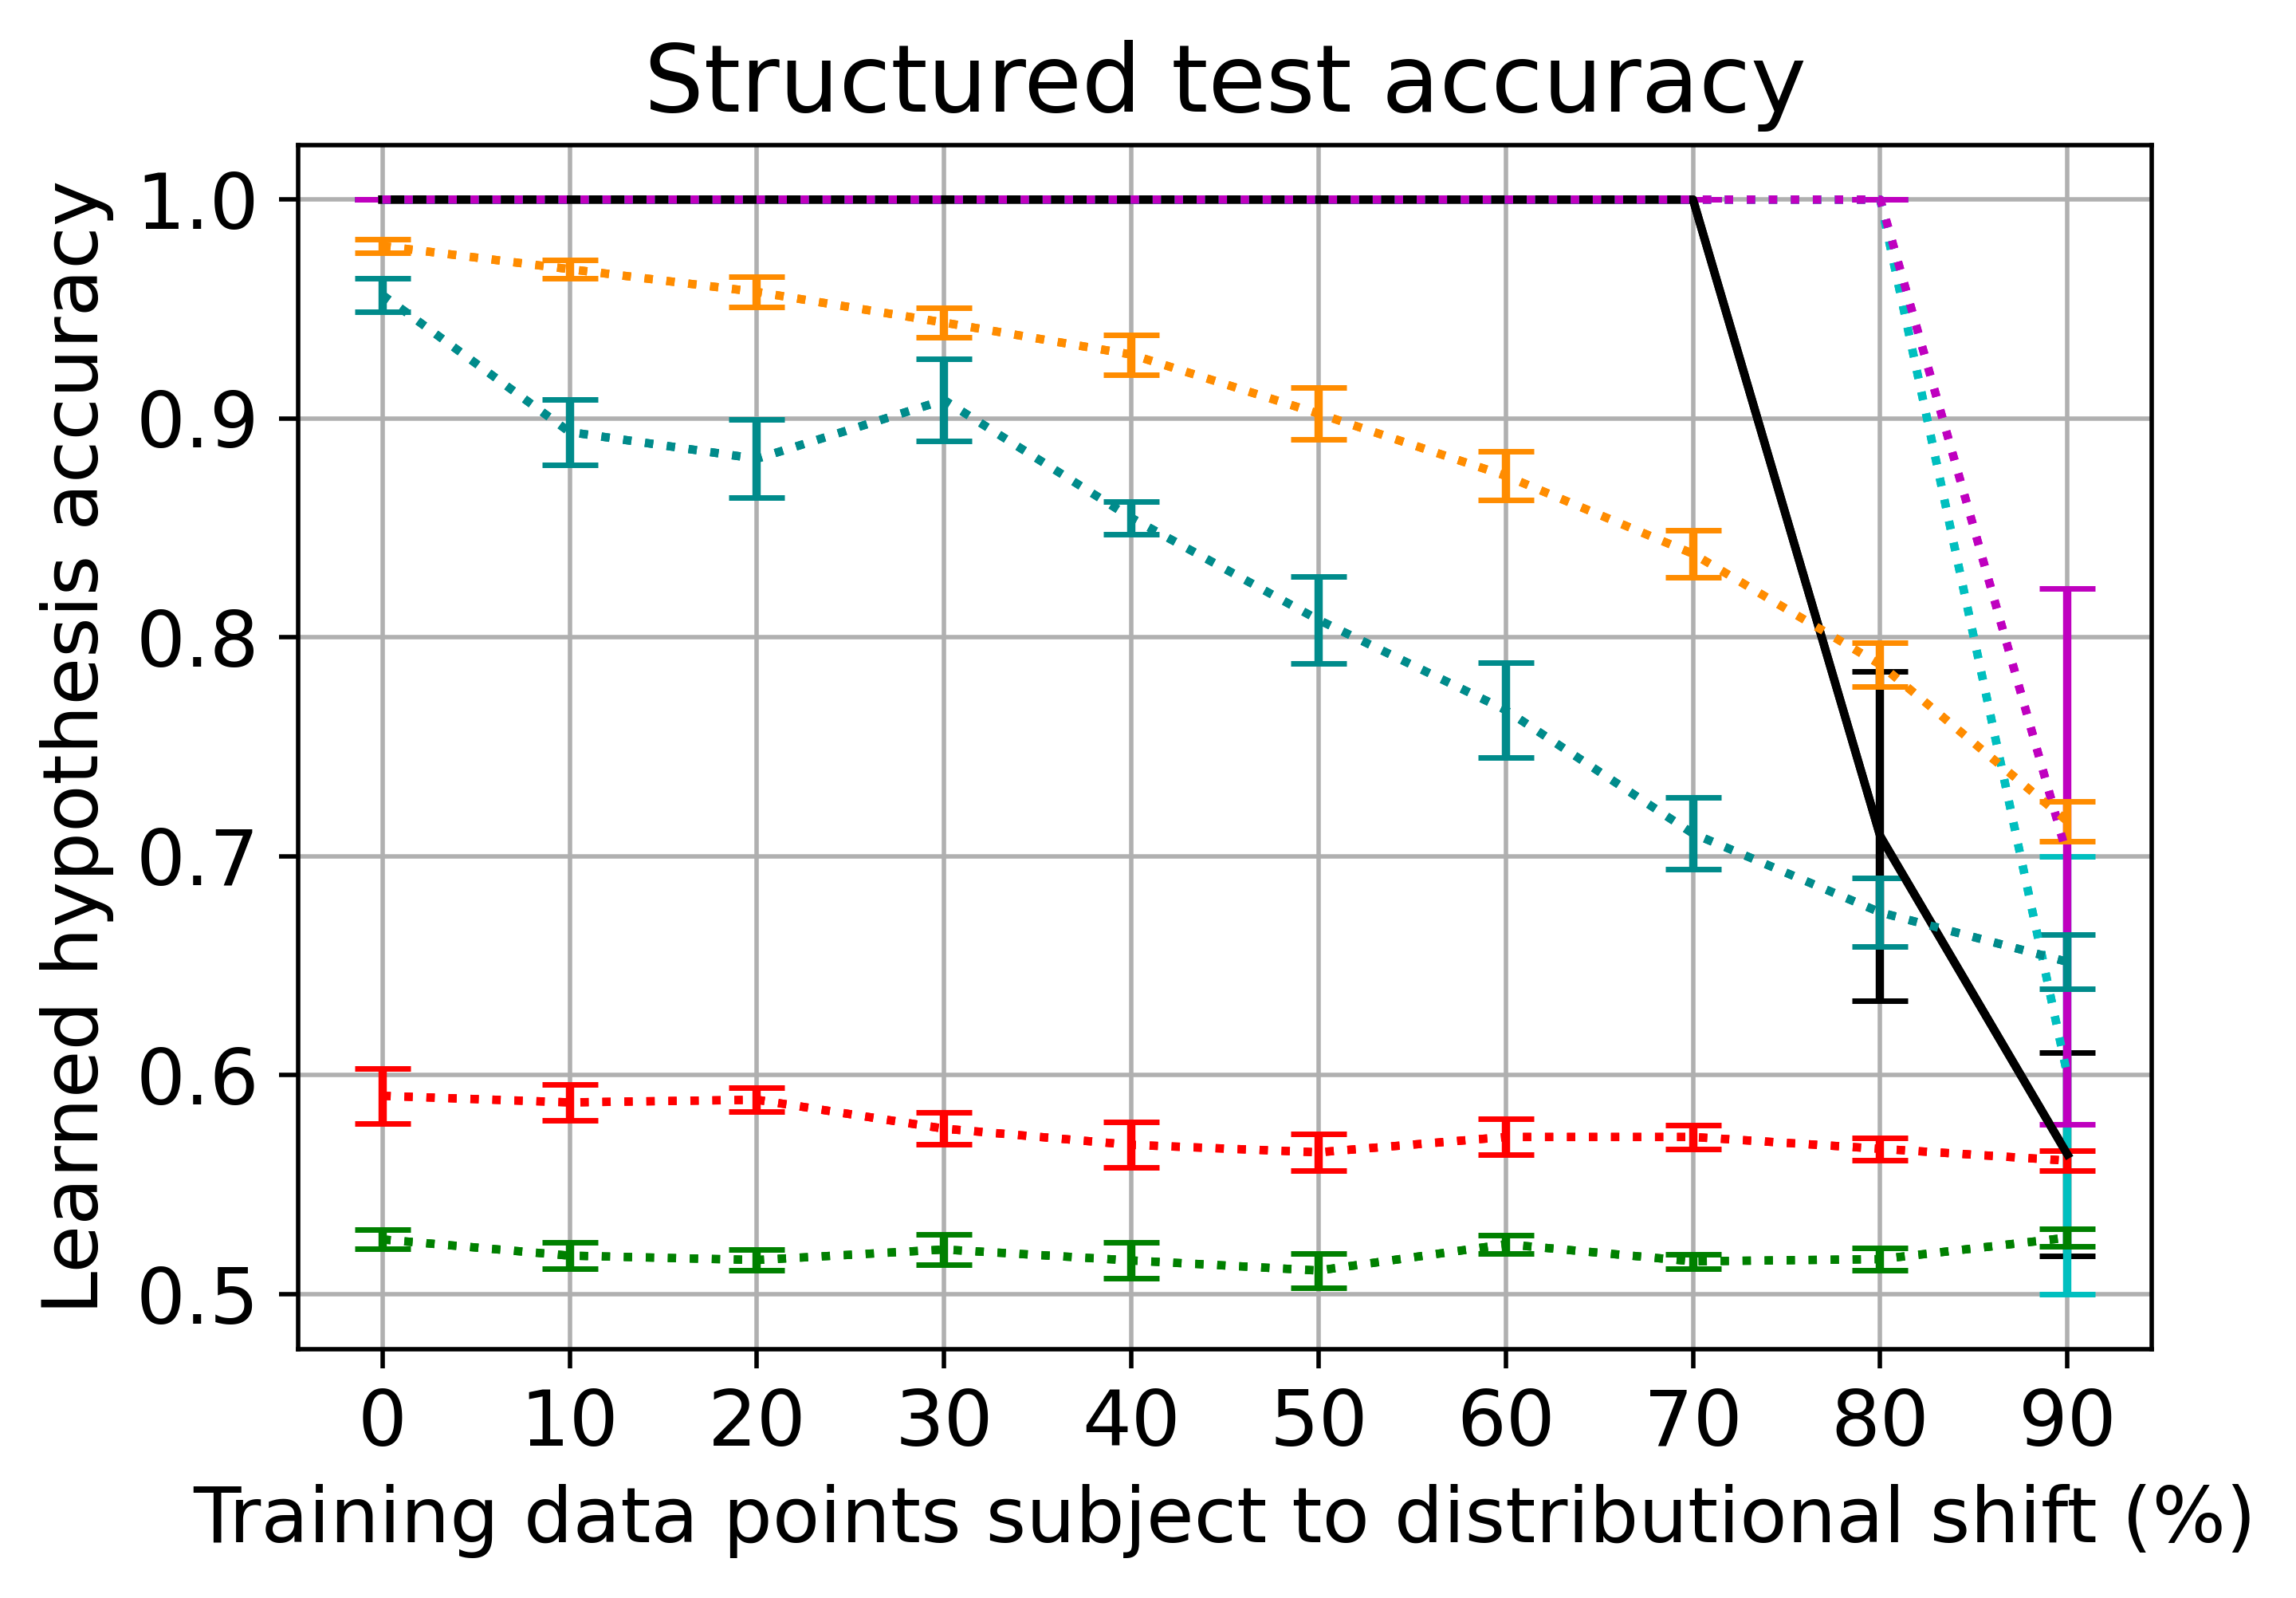
\includegraphics[width=\textwidth]{logic-based-classification/sudoku_4x4_structured_test_data_results.png}
\label{sudoku4x4-results}
\end{figure}



The results for sudoku 9x9 are shown in figure \ref{sudoku9x9-results}
\begin{figure}[h]
\caption{A comparison of the sudoku 4x4 task performance with increasing level of distribution shifts}
\centering
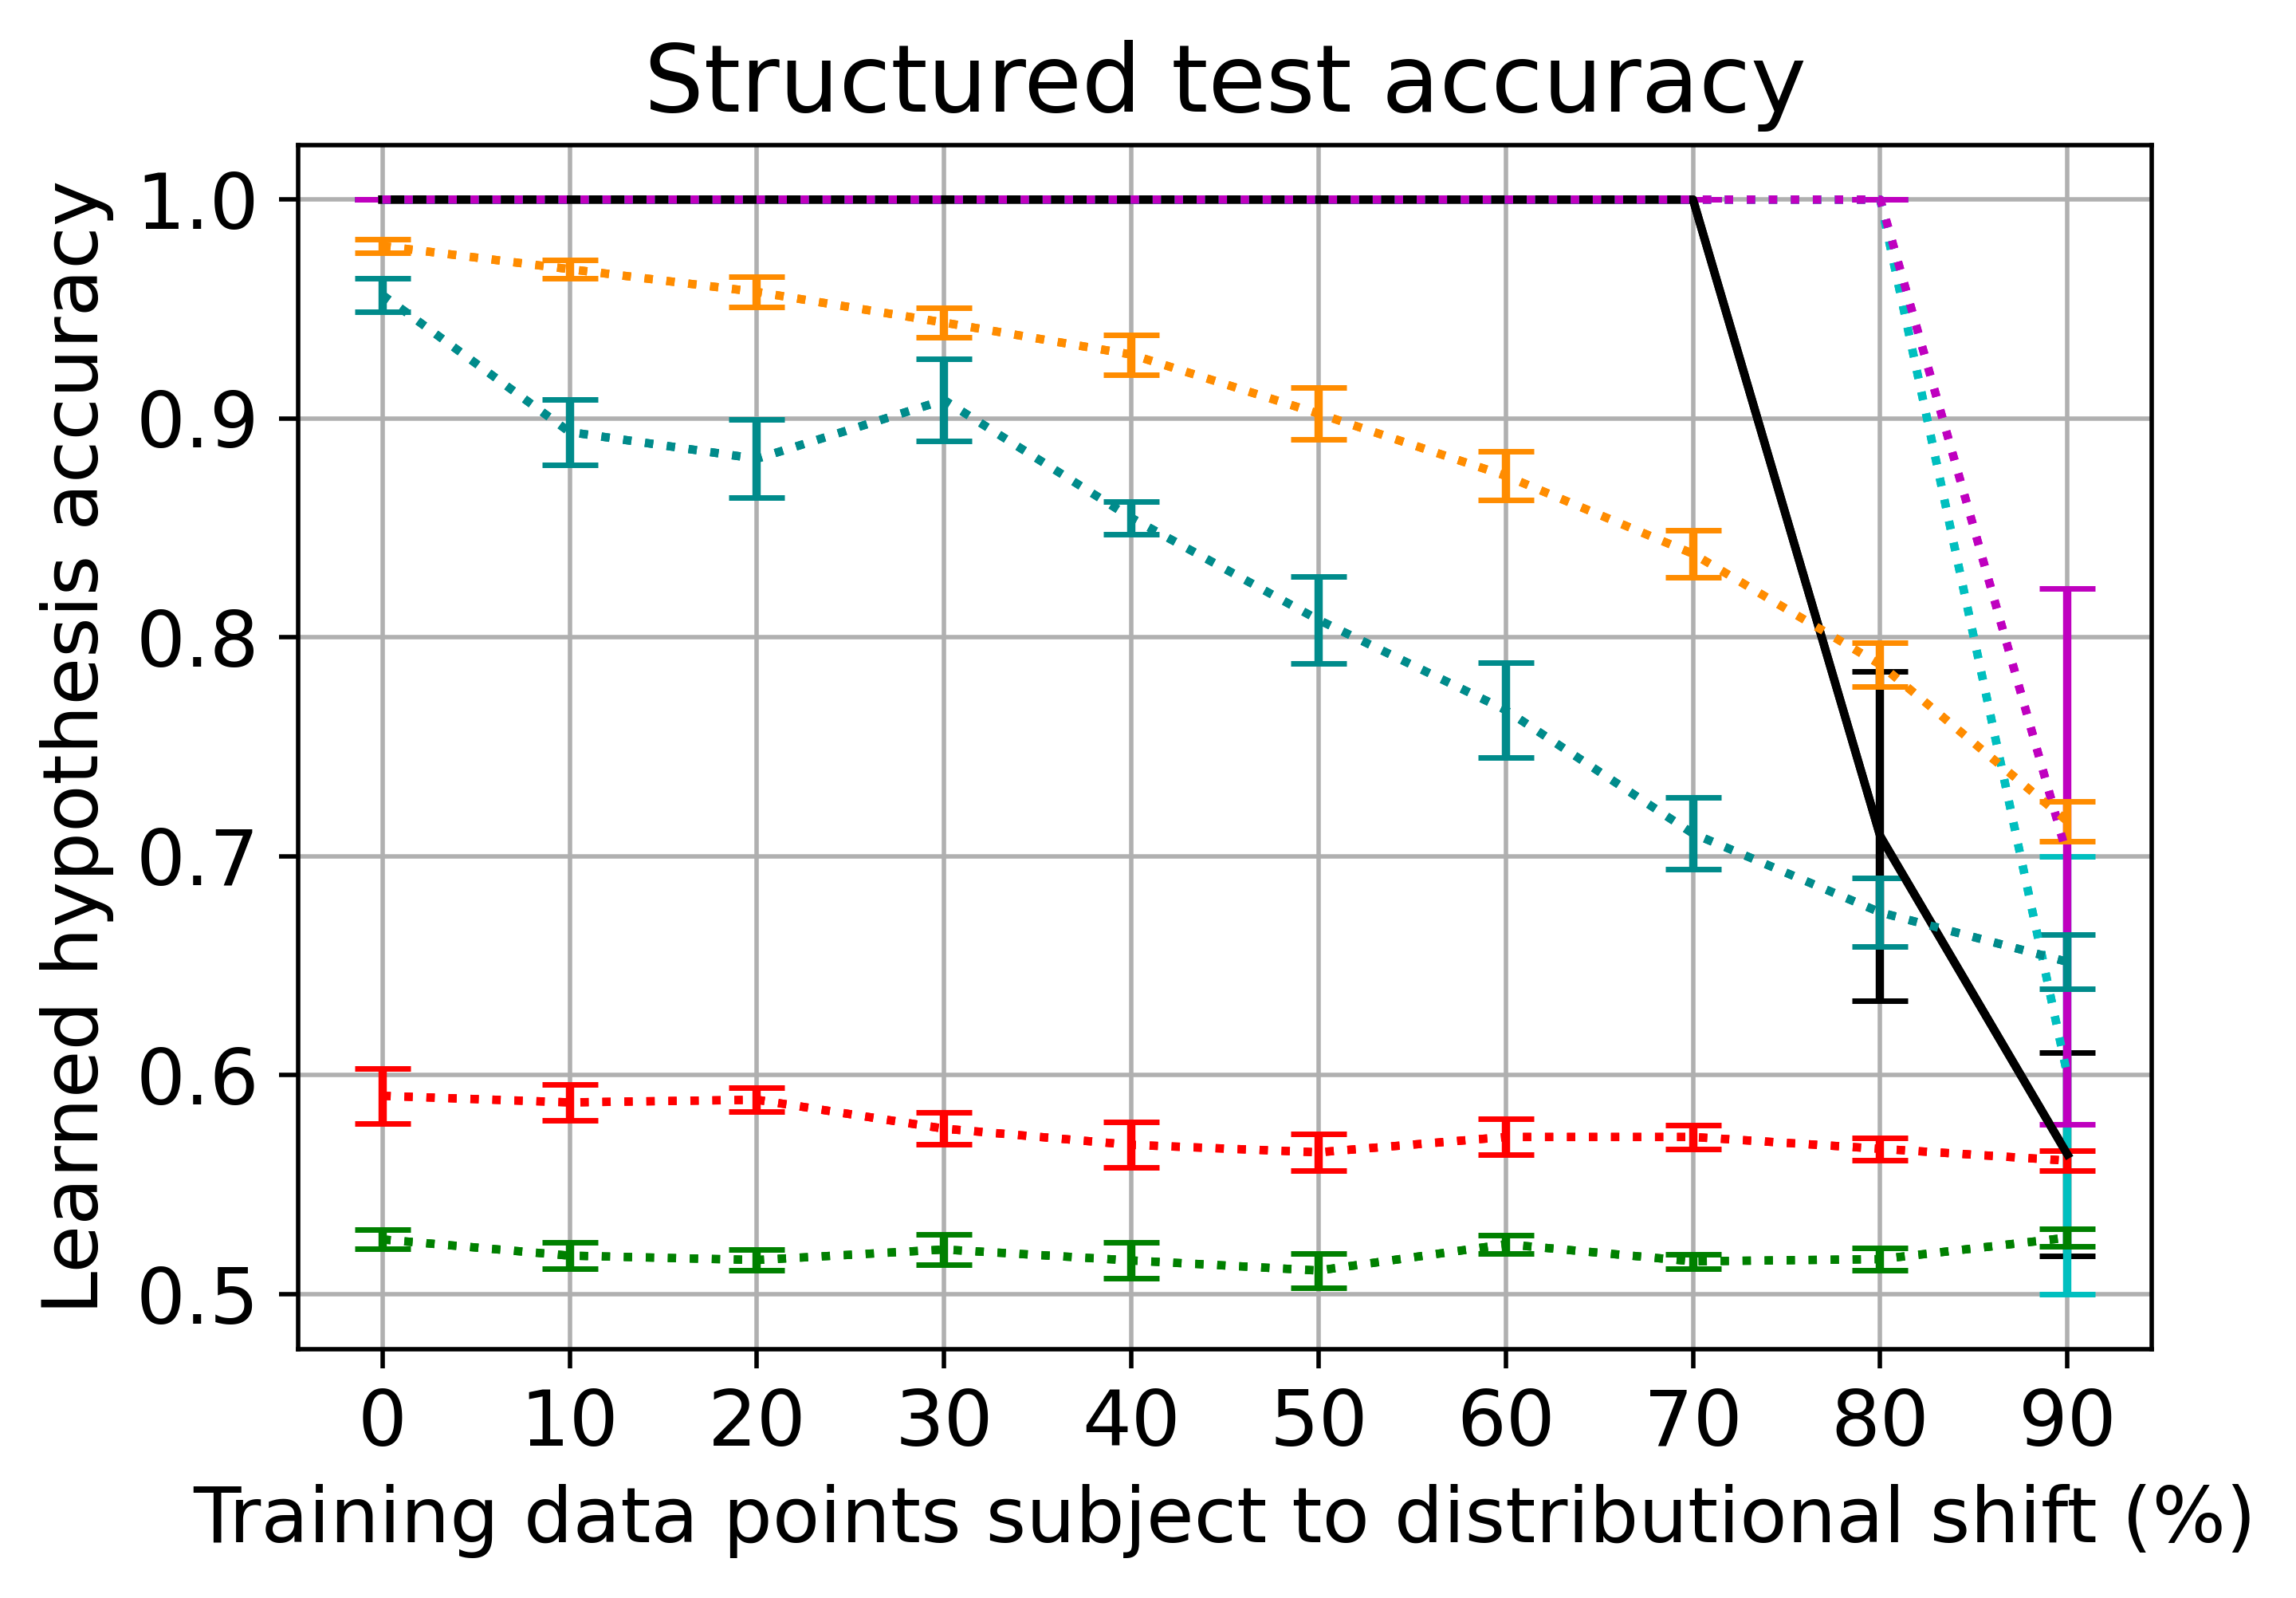
\includegraphics[width=\textwidth]{logic-based-classification/sudoku_4x4_structured_test_data_results.png}
\label{sudoku9x9-results}
\end{figure}


All in all, the Prob-FF-NSL generally performs well, having a perfect true test score in spite of 70\% of examples under a distribution shift.
However, it performs worse than the FF-NSL method on this particular task. 
The reason for it is the higher importance the FF-NSL assigns to the train examples that are not under the distribution shift.
It may be useful to integrate a similar notion of example importance to the Prob-NSL approach too.


\subsection{Concept Bottleneck Pipeline}

We also test the presented Prob-NSL framework within the context of a concept bottleneck model.
The architecture that the Prob-NSL model used for this task is presented in \ref{change-to-the-concept-bottleneck-architecture}.

As baselines, we compare the model to an end-to-end network and the concept bottleneck model with identical architectures.
The latter is the same model that is used for the concept prediction for the Prob-NSL model.

Their results are summarised in the table below:

\begin{center}
\begin{tabular}{ |M{3cm}||M{3cm}|M{3cm}|M{3cm}|  }
 \hline
 \multicolumn{4}{|c|}{Accuracy Comparison} \\
 \hline
 \hline
  & End-to-end model&Concept bottleneck model & Prob-NSL concept bottleneck \\ 
 \hline
 Train & X $\pm$ X & X $\pm$ X & 0.922 $\pm$ 0.021 \\
 Test & 0.687 $\pm$ 0.004 & 0.685 $\pm$ 0.005 & 0.910 $\pm$ 0.023 \\
 \hline
\end{tabular}
\end{center}

The Prob-NSL model greatly outperforms the other two with ~33\% test higher test set accuracy.
The results could have been even higher if there the concept bottleneck model is able to distinguish between \emph{strike} and \emph{ball} well.
In some instances, the model predicts a \emph{strike} in every case where there is a \emph{strike}.
When the model learns well enough to distinguish between the two, the accuracy jumps to values as high as 96\%.

\section{Discussion}

The proposed logic based classification method, working extremely well as a part of the concept bottleneck pipeline.
It outperforms the approach from Chapter \ref{concept-bottleneck-pipeline}.

% INSERT Online Symbolic Learning of Policies for Explainable Security reference
The method could be further improved, such as setting different penalties on examples that we care more about being satisfied.
Moreover, the approach for choosing a prior chosen may not be flexible enough for all possible applications.
Incorporating the configurable prior approach shown in X would have a lot of benefit for some applications.

% TODO: Luke feedback -random forest -feature importance - how often a predicate gets used to make a prediction 